\documentclass[
	%parspace, % Add vertical space between paragraphs
	%noindent, % No indentation of first lines in each paragraph
	%nohyp, % No hyphenation of words
	%twoside, % Double sided format
	%draft, % Quicker draft compilation without rendering images
	%final, % Set final to hide todos
]{elteikthesis}[2024/04/26]

% The minted package is also supported for source highlighting
% See elteikthesis_minted.tex for example
%\usepackage[newfloat]{minted}

% Document's metadata
\title{NutriFit: A Comprehensive Health and Fitness Tracking Application} % title
\date{2026} % year of defense

% Author's metadata
\author{[Your Full Name]} % Replace with your name
\degree{Computer Science BSc} % Or your degree program

% Supervisor(s)' metadata
\supervisor{[Supervisor's Name]} % Replace with supervisor's name
\affiliation{[Supervisor's Title]} % Replace with supervisor's title
%\extsupervisor{Jane Doe} % external supervisor's name (if applicable)
%\extaffiliation{Senior Developer} % external supervisor's affiliation

% University's metadata
\university{Eötvös Loránd University} % university's name
\faculty{Faculty of Informatics} % faculty's name
\department{Dept. of Software Technology and Methodology} % department's name
\city{Budapest} % city
\logo{elte_cimer_szines} % logo

% Add bibliography file
\addbibresource{references.bib}

% The document
\begin{document}

% Set document language
%\documentlang{hungarian}
\documentlang{english}

% List of todos (not in the final document)
%\listoftodos[\todolabel]

% Title page (mandatory)
\maketitle

% Topic declaration page (mandatory) - can also be attached instead
% Option 1: Include as image
% Topic Registration Form
\thispagestyle{empty}

\begin{center}
    {\Large \textbf{Topic Registration Form}}
\end{center}

\vspace{1cm}

% Add scanned image of registration form
\begin{figure}[H]
    \centering
    \includegraphics[width=0.9\textwidth]{images/registration-form.png}
    \caption*{Topic Registration Form}
\end{figure}

\newpage

% Option 2: Attach physical copy instead
%\includepdf{topicdeclaration.pdf}

% Acknowledgements (optional)
\chapter*{\acklabel}
\addcontentsline{toc}{chapter}{\acklabel}
% Acknowledgements
\chapter*{Acknowledgements}
\addcontentsline{toc}{chapter}{Acknowledgements}

I would like to express my sincere gratitude to my supervisor, [Supervisor Name], for their invaluable guidance, continuous support, and insightful feedback throughout the development of this thesis project. Their expertise and encouragement were instrumental in shaping this work.

I am also grateful to the Faculty of Informatics at Eötvös Loránd University for providing the necessary resources and academic environment that made this research possible.

Special thanks to my family and friends for their unwavering support and understanding during the challenging phases of this project.

Finally, I would like to acknowledge the open-source community, particularly the developers of Next.js, React, Prisma, and other technologies used in this project, whose contributions made the implementation of this system feasible.

\vspace{1cm}

\begin{flushright}
[Your Name]\\
Budapest, 2026
\end{flushright}

\newpage

\cleardoublepage

% Abstract
\chapter*{Abstract}
\addcontentsline{toc}{chapter}{Abstract}
% Abstract
\chapter*{Abstract}
\addcontentsline{toc}{chapter}{Abstract}

This thesis presents the design, development, and implementation of NutriFit, a comprehensive web-based Health and Fitness Management System. The system addresses the growing need for personalized health tracking and management tools in an increasingly health-conscious society.

NutriFit provides users with an integrated platform to manage their nutrition, fitness activities, and health goals. The system features personalized diet plan generation, workout plan creation, meal and exercise logging, progress tracking with visual analytics, and goal management capabilities. Built using modern web technologies including Next.js 14, React, TypeScript, and Prisma ORM with SQLite database, the system ensures type safety, scalability, and maintainability.

The development methodology followed an iterative approach with continuous testing and refinement. The system implements secure user authentication using JWT tokens, comprehensive input validation, and responsive design principles to ensure accessibility across different devices. Special attention was given to user experience, with features like real-time form validation, password strength indicators, and interactive data visualizations using Recharts library.

Testing was conducted at multiple levels including unit tests, integration tests, and end-to-end functional testing. The system successfully passed 28 automated test cases covering authentication, health profile management, diet plan generation, and water intake tracking functionalities. Performance optimization techniques were implemented, including database indexing, parallel API calls, and client-side caching, resulting in improved response times and user experience.

The thesis demonstrates the practical application of modern web development practices, database design principles, and software engineering methodologies. The system provides a solid foundation for future enhancements including mobile application development, integration with wearable devices, and advanced machine learning-based recommendations.

\textbf{Keywords:} Health Management, Fitness Tracking, Web Application, Next.js, React, TypeScript, Prisma ORM, Personalized Nutrition, Workout Planning, Progress Analytics

\newpage

\cleardoublepage

% Table of contents (mandatory)
\tableofcontents
\cleardoublepage

% Main content - 4 Chapters
% Chapter 1: Introduction
\chapter{Introduction}

\section{Background and Motivation}

In recent years, there has been a significant increase in health consciousness among individuals worldwide. The World Health Organization reports that lifestyle-related diseases such as obesity, diabetes, and cardiovascular conditions are on the rise, largely due to poor dietary habits and sedentary lifestyles. This growing concern has created a demand for accessible, user-friendly tools that can help individuals monitor and improve their health and fitness.

Traditional methods of health tracking, such as manual food diaries and paper-based workout logs, are often cumbersome and difficult to maintain consistently. Moreover, they lack the analytical capabilities needed to provide meaningful insights into one's health progress. While numerous health and fitness applications exist in the market, many suffer from complexity, lack of personalization, or focus on only one aspect of health management.

The motivation behind developing NutriFit stems from the need for an integrated, comprehensive solution that combines nutrition tracking, fitness management, and progress analytics in a single, intuitive platform. The system aims to empower users to take control of their health journey by providing personalized recommendations, easy-to-use logging features, and visual progress tracking.

\section{Problem Statement}

Despite the availability of various health and fitness applications, several challenges persist in the domain of personal health management. First, many existing solutions require users to navigate multiple platforms to track different aspects of their health, leading to fragmented data and inconsistent usage. Second, the lack of personalization in diet and workout recommendations often results in generic advice that may not suit individual needs, preferences, or health conditions. Third, complex user interfaces and steep learning curves discourage consistent usage, particularly among users who are not tech-savvy.

Additionally, many applications fail to provide comprehensive progress tracking and analytics, making it difficult for users to understand their health trends and make informed decisions. The absence of proper allergen management and dietary restriction features can also pose health risks for users with specific nutritional requirements.

This thesis addresses these challenges by developing NutriFit, a web-based system that provides an integrated approach to health and fitness management with emphasis on personalization, user experience, and comprehensive tracking capabilities.

\section{Objectives of the Study}

The primary objectives of this thesis are as follows:

\begin{enumerate}
    \item To design and develop a comprehensive web-based health and fitness management system that integrates nutrition tracking, workout planning, and progress analytics in a single platform.
    
    \item To implement personalized diet and workout plan generation algorithms that consider user-specific parameters such as age, weight, height, activity level, dietary restrictions, and health goals.
    
    \item To create an intuitive and responsive user interface that ensures ease of use across different devices and promotes consistent user engagement.
    
    \item To develop a robust database schema that efficiently stores and manages user data, health profiles, meal logs, exercise logs, and generated plans while maintaining data integrity and security.
    
    \item To implement comprehensive testing strategies including unit tests, integration tests, and functional tests to ensure system reliability and correctness.
\end{enumerate}

\section{Scope of the Study}

This thesis encompasses the complete software development lifecycle of the NutriFit system, from requirements analysis to implementation and testing. The scope includes the following key areas:

\textbf{Functional Scope:}
\begin{itemize}
    \item User authentication and authorization system with secure password management
    \item Health profile management with comprehensive user information
    \item Personalized diet plan generation based on caloric needs and dietary restrictions
    \item Customized workout plan creation considering fitness level and goals
    \item Meal and exercise logging with detailed nutritional and activity tracking
    \item Progress analytics with visual representations of health trends
    \item Goal setting and tracking functionality
    \item Water intake monitoring
    \item Favorite foods and exercises management
\end{itemize}

\textbf{Technical Scope:}
\begin{itemize}
    \item Frontend development using Next.js 14, React, and TypeScript
    \item Backend API development using Next.js API routes
    \item Database design and implementation using Prisma ORM with SQLite
    \item Authentication implementation using JWT tokens
    \item Responsive UI design using Tailwind CSS
    \item Data visualization using Recharts library
    \item Automated testing using Jest and React Testing Library
\end{itemize}

\textbf{Limitations:}
The system is designed as a web application and does not include native mobile applications. Integration with wearable devices and external health APIs is not covered in this version. Advanced machine learning-based recommendations and social features are considered as future enhancements.

\section{Methodology Overview}

The development of NutriFit followed an iterative and incremental approach, combining elements of agile methodology with structured software engineering practices. The methodology consisted of the following phases:

\textbf{Requirements Analysis:} Initial phase involved identifying user needs, defining functional and non-functional requirements, and establishing system objectives. This included studying existing health and fitness applications to understand common features and identify gaps.

\textbf{System Design:} Comprehensive system architecture was designed, including database schema, API structure, and user interface mockups. Entity-Relationship diagrams, use case diagrams, and class diagrams were created to visualize system components and their interactions.

\textbf{Implementation:} Development was carried out in iterative cycles, with each cycle focusing on specific features. The implementation prioritized core functionalities such as authentication and health profile management, followed by plan generation, logging features, and analytics.

\textbf{Testing:} Continuous testing was performed throughout the development process. Unit tests were written for individual components, integration tests verified API endpoints, and functional tests ensured end-to-end feature correctness. A total of 28 automated test cases were implemented and successfully executed.

\textbf{Refinement:} Based on testing results and usability considerations, the system underwent multiple refinement iterations to improve performance, user experience, and code quality.

\section{Structure of the Thesis}

This thesis is organized into four main chapters:

\textbf{Chapter 1: Introduction} provides the background, motivation, problem statement, objectives, scope, and methodology overview of the project.

\textbf{Chapter 2: User Documentation} describes the system from the user's perspective, including system requirements, installation procedures, user interface overview, and detailed functional descriptions of all features.

\textbf{Chapter 3: Developer Documentation} presents the technical aspects of the system, including system architecture, technologies used, database design, application components, security measures, testing approach, and implementation details.

\textbf{Chapter 4: Summary} concludes the thesis by summarizing the development process, system functionality, testing results, achievements, and potential future enhancements.

The thesis also includes comprehensive lists of figures, tables, code listings, and abbreviations to facilitate navigation and understanding of the technical content.

\cleardoublepage

% Chapter 2: User Documentation
\chapter{User Documentation}

\section{Introduction}

NutriFit is a comprehensive web-based Health and Fitness Management System designed to help users track their nutrition, manage workout routines, and monitor their health progress. The system provides an integrated platform where users can create personalized diet and workout plans, log their daily meals and exercises, set health goals, and visualize their progress through interactive charts and analytics.

The application is built using modern web technologies to ensure a responsive, fast, and user-friendly experience across different devices including desktops, tablets, and smartphones. Figure \ref{fig:framework} illustrates the overall framework and technology stack used in the NutriFit system.

\begin{figure}[H]
    \centering
    \includegraphics[width=0.9\textwidth]{images/framework-diagram.png}
    \caption{NutriFit System Framework and Technology Stack}
    \label{fig:framework}
\end{figure}

The framework diagram shown in Figure \ref{fig:framework} demonstrates the layered architecture of the system. At the presentation layer, the system uses Next.js 14 with React for building the user interface, styled with Tailwind CSS for responsive design. The application layer consists of Next.js API routes that handle business logic and data processing. The data layer utilizes Prisma ORM for database operations with SQLite as the database engine. Additional libraries such as Recharts for data visualization, JWT for authentication, and Bcrypt for password hashing complete the technology stack.

\section{System Requirements}

To run and use the NutriFit system, the following requirements must be met:

\subsection{Hardware Requirements}
\begin{itemize}
    \item \textbf{Processor:} Intel Core i3 or equivalent (minimum), Intel Core i5 or better (recommended)
    \item \textbf{RAM:} 4 GB (minimum), 8 GB or more (recommended)
    \item \textbf{Storage:} 500 MB free disk space for application and database
    \item \textbf{Display:} 1366x768 resolution (minimum), 1920x1080 or higher (recommended)
    \item \textbf{Network:} Internet connection for initial setup and updates
\end{itemize}

\subsection{Software Requirements}
\begin{itemize}
    \item \textbf{Operating System:} Windows 10/11, macOS 10.15+, or Linux (Ubuntu 20.04+)
    \item \textbf{Node.js:} Version 18.0 or higher
    \item \textbf{npm:} Version 9.0 or higher (comes with Node.js)
    \item \textbf{Web Browser:} Google Chrome 90+, Firefox 88+, Safari 14+, or Edge 90+
\end{itemize}

\subsection{User Requirements}
\begin{itemize}
    \item Basic computer literacy and web browsing skills
    \item Valid email address for account registration
    \item Understanding of basic health and fitness concepts
\end{itemize}

\section{Installation and Setup}

This section provides step-by-step instructions for installing and setting up the NutriFit system on a local machine.

\subsection{Installation Steps}

\textbf{Step 1: Install Node.js}

Download and install Node.js from the official website (https://nodejs.org). Verify the installation by opening a terminal or command prompt and running:

\begin{lstlisting}[language=bash, caption=Verify Node.js Installation]
node --version
npm --version
\end{lstlisting}

\textbf{Step 2: Clone or Download the Project}

Obtain the NutriFit project files either by cloning from a repository or extracting from a provided archive.

\textbf{Step 3: Install Dependencies}

Navigate to the project directory and install required packages:

\begin{lstlisting}[language=bash, caption=Install Project Dependencies]
cd nutrifit
npm install
\end{lstlisting}

\textbf{Step 4: Configure Environment Variables}

Create a \texttt{.env} file in the project root directory with the following configuration:

\begin{lstlisting}[caption=Environment Configuration]
DATABASE_URL="file:./prisma/dev.db"
JWT_SECRET="your-secret-key-here"
NODE_ENV="development"
\end{lstlisting}

\textbf{Step 5: Initialize Database}

Set up the database schema and seed initial data:

\begin{lstlisting}[language=bash, caption=Database Setup]
npx prisma generate
npx prisma migrate deploy
npx tsx prisma/seed.ts
\end{lstlisting}

\textbf{Step 6: Start the Development Server}

Launch the application:

\begin{lstlisting}[language=bash, caption=Start Application]
npm run dev
\end{lstlisting}

The application will be accessible at \texttt{http://localhost:3000}.

\section{User Interface Overview}

The NutriFit user interface is designed with simplicity and usability in mind. The system follows a consistent design pattern across all pages, featuring a clean layout, intuitive navigation, and responsive design that adapts to different screen sizes.

\subsection{Landing Page}

Figure \ref{fig:landing} shows the landing page, which serves as the entry point for new and returning users. The page features a hero section with the NutriFit branding, key features overview, and call-to-action buttons for registration and login.

\begin{figure}[H]
    \centering
    \includegraphics[width=0.9\textwidth]{images/landing-page.png}
    \caption{NutriFit Landing Page}
    \label{fig:landing}
\end{figure}

The landing page displayed in Figure \ref{fig:landing} presents a modern and welcoming interface with a gradient background featuring the NutriFit logo prominently at the top. The main heading "Transform Your Health Journey" immediately communicates the system's purpose. Below the heading, three key features are highlighted with icons: personalized nutrition plans, custom workout routines, and progress tracking. The page includes two prominent buttons for "Get Started" and "Sign In" to guide users toward registration or login.

\subsection{Dashboard}

After logging in, users are directed to the main dashboard shown in Figure \ref{fig:dashboard}. The dashboard provides an overview of the user's health status, recent activities, and quick access to all major features.

\begin{figure}[H]
    \centering
    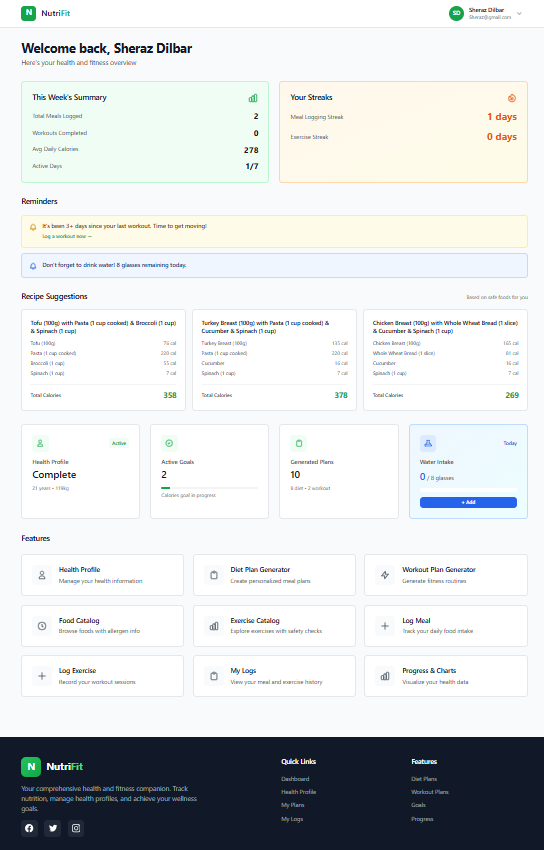
\includegraphics[width=0.9\textwidth]{images/dashboard.png}
    \caption{Main Dashboard Interface}
    \label{fig:dashboard}
\end{figure}

The dashboard interface in Figure \ref{fig:dashboard} features a navigation bar at the top with the NutriFit logo and user profile menu. The main content area displays summary cards showing today's calorie intake, workouts completed, water intake, and active goals. Below the summary cards, quick action buttons provide direct access to key features such as logging meals, logging exercises, generating diet plans, and creating workout plans. The dashboard also includes a recent activity section showing the user's latest logged meals and exercises.

\section{Functional Description}

This section describes each functional feature of the NutriFit system in detail, including screenshots and usage instructions.

\subsection{User Registration}

The registration feature allows new users to create an account in the system. Figure \ref{fig:register} shows the registration page interface.

\begin{figure}[H]
    \centering
    \includegraphics[width=0.8\textwidth]{images/register-page.png}
    \caption{User Registration Page}
    \label{fig:register}
\end{figure}

The registration page shown in Figure \ref{fig:register} features a split-screen design with branding information on the left and the registration form on the right. The form includes fields for full name, email address, password, and password confirmation. A notable feature is the password strength indicator that appears below the password field, displaying a visual representation of password strength using colored bars. The indicator shows "Weak," "Medium," or "Strong" based on password complexity, helping users create secure passwords. Real-time validation provides immediate feedback on input errors, such as invalid email format or password mismatch. Upon successful registration, users are automatically logged in and redirected to the dashboard.

\subsection{User Login}

The login feature provides secure access to existing user accounts. Figure \ref{fig:login} displays the login page interface.

\begin{figure}[H]
    \centering
    \includegraphics[width=0.8\textwidth]{images/login-page.png}
    \caption{User Login Page}
    \label{fig:login}
\end{figure}

The login page illustrated in Figure \ref{fig:login} maintains the same split-screen design as the registration page for consistency. The left side features motivational text and key benefits of using NutriFit, while the right side contains the login form with email and password fields. The form includes a "Remember Me" checkbox for convenience and a "Forgot Password" link for account recovery. Error messages are displayed prominently when login credentials are incorrect, and successful authentication redirects users to the dashboard with their session maintained using JWT tokens.

\subsection{Health Profile Management}

Users can create and manage their health profiles, which serve as the foundation for personalized recommendations. Figure \ref{fig:health-profile} shows the health profile creation interface.

\begin{figure}[H]
    \centering
    \includegraphics[width=0.9\textwidth]{images/health-profile.png}
    \caption{Health Profile Management Interface}
    \label{fig:health-profile}
\end{figure}

The health profile management interface in Figure \ref{fig:health-profile} provides a comprehensive form for users to input their personal health information. The form is organized into logical sections including basic information (age, gender, height, weight), activity level selection (sedentary, lightly active, moderately active, very active, extremely active), health goals (weight loss, weight gain, muscle gain, maintenance), and dietary restrictions. The allergen selection feature allows users to specify multiple allergens from a predefined list including milk, eggs, fish, shellfish, tree nuts, peanuts, wheat, soy, and gluten. The system uses this information to calculate BMI, determine caloric needs, and generate personalized diet and workout plans. The interface includes helpful tooltips and validation messages to guide users in providing accurate information.

\subsection{Diet Plan Generation}

The diet plan generation feature creates personalized meal plans based on user health profiles and preferences. Figure \ref{fig:diet-plan} illustrates the diet plan generation interface.

\begin{figure}[H]
    \centering
    \includegraphics[width=0.9\textwidth]{images/diet-plan-generation.png}
    \caption{Diet Plan Generation Interface}
    \label{fig:diet-plan}
\end{figure}

The diet plan generation interface shown in Figure \ref{fig:diet-plan} allows users to customize their meal plan parameters. Users can select the plan duration (7, 14, or 30 days), target daily calorie intake, number of meals per day (3, 4, or 5), and specific dietary goals. The system automatically suggests calorie targets based on the user's health profile but allows manual adjustment. Upon generation, the system creates a detailed meal plan that respects the user's allergen restrictions and dietary preferences. Each meal includes food items from the database with appropriate serving sizes to meet the calorie target. The generated plan is displayed in a structured format showing breakfast, lunch, dinner, and optional snacks with total calorie counts for each meal.

\subsection{Workout Plan Generation}

The workout plan generation feature creates customized exercise routines tailored to user fitness levels and goals. Figure \ref{fig:workout-plan} shows the workout plan generation interface.

\begin{figure}[H]
    \centering
    \includegraphics[width=0.9\textwidth]{images/workout-plan-generation.png}
    \caption{Workout Plan Generation Interface}
    \label{fig:workout-plan}
\end{figure}

The workout plan generation interface displayed in Figure \ref{fig:workout-plan} provides options for users to specify their workout preferences. Users can select the plan duration, workout intensity level (beginner, intermediate, advanced), focus area (full body, upper body, lower body, cardio, strength), and days per week for training. The system generates a structured workout plan that includes a variety of exercises from the database, organized by day and muscle group. Each exercise entry specifies the number of sets, repetitions, and estimated duration. The plan considers the user's fitness level to ensure appropriate exercise selection and intensity, preventing injury while promoting progress toward fitness goals.

\subsection{Meal Logging}

The meal logging feature allows users to record their daily food intake for tracking and analysis. Figure \ref{fig:meal-log} illustrates the meal logging interface.

\begin{figure}[H]
    \centering
    \includegraphics[width=0.9\textwidth]{images/meal-logging.png}
    \caption{Meal Logging Interface}
    \label{fig:meal-log}
\end{figure}

The meal logging interface shown in Figure \ref{fig:meal-log} provides an intuitive way to record meals throughout the day. Users can search for food items from the comprehensive food database, which includes nutritional information for each item. The search functionality supports partial matching and displays results in categorized groups (fruits, vegetables, proteins, grains, dairy, nuts, snacks). Users can select multiple food items, specify quantities, and assign them to meal types (breakfast, lunch, dinner, snack). The interface displays a running total of calories for the selected foods, helping users stay within their daily calorie targets. Each logged meal is timestamped and stored in the database for future reference and analysis.

\subsection{Exercise Logging}

The exercise logging feature enables users to track their workout activities and physical exercises. Figure \ref{fig:exercise-log} shows the exercise logging interface.

\begin{figure}[H]
    \centering
    \includegraphics[width=0.9\textwidth]{images/exercise-logging.png}
    \caption{Exercise Logging Interface}
    \label{fig:exercise-log}
\end{figure}

The exercise logging interface illustrated in Figure \ref{fig:exercise-log} allows users to record their workout sessions with detailed information. Users can search and select exercises from the database, which includes various types of activities such as cardio, strength training, flexibility exercises, and sports. For each exercise, users can specify the duration, number of sets and repetitions (for strength exercises), and intensity level. The interface calculates estimated calories burned based on the exercise type and duration. Users can log multiple exercises in a single session, and the system maintains a complete history of all workout activities for progress tracking and analysis.

\subsection{Progress Tracking and Analytics}

The progress tracking feature provides visual analytics of user health data over time. Figure \ref{fig:progress} displays the progress analytics interface.

\begin{figure}[H]
    \centering
    \includegraphics[width=0.9\textwidth]{images/progress-analytics.png}
    \caption{Progress Tracking and Analytics Interface}
    \label{fig:progress}
\end{figure}

The progress analytics interface shown in Figure \ref{fig:progress} presents comprehensive visualizations of user health data. The page includes summary statistics cards displaying total meals logged, workouts completed, average daily calories, and days tracked. Interactive charts show daily calorie intake trends using a line chart, daily workout frequency using a bar chart, and food category distribution using a pie chart. Users can select different time ranges (7 days or 30 days) to view their progress over various periods. The interface also includes a key insights section that provides personalized feedback based on the user's activity patterns. All charts are interactive, allowing users to hover over data points for detailed information. The page includes export functionality to download progress data in CSV format and print functionality to generate physical reports.

\subsection{Goal Management}

The goal management feature allows users to set, track, and manage their health and fitness goals. Figure \ref{fig:goals} shows the goal management interface.

\begin{figure}[H]
    \centering
    \includegraphics[width=0.9\textwidth]{images/goal-management.png}
    \caption{Goal Management Interface}
    \label{fig:goals}
\end{figure}

The goal management interface displayed in Figure \ref{fig:goals} enables users to create specific, measurable health goals. Users can set goals for weight targets, daily calorie intake, weekly workout frequency, water intake, or custom objectives. Each goal includes a title, description, target value, current progress, and deadline. The interface displays goals in organized cards showing progress bars and completion percentages. Users can mark goals as completed, edit existing goals, or delete goals that are no longer relevant. The system tracks goal progress automatically based on logged meals, exercises, and other activities, providing real-time updates on achievement status.

\subsection{Water Intake Tracking}

The water intake tracking feature helps users monitor their daily hydration levels. Figure \ref{fig:water} illustrates the water intake tracking interface.

\begin{figure}[H]
    \centering
    \includegraphics[width=0.8\textwidth]{images/water-intake.png}
    \caption{Water Intake Tracking Interface}
    \label{fig:water}
\end{figure}

The water intake tracking interface shown in Figure \ref{fig:water} provides a simple and effective way to log daily water consumption. Users can quickly add water intake in standard serving sizes (250ml glasses) with a single click. The interface displays a visual progress indicator showing the percentage of daily water goal achieved, along with the total amount consumed in milliliters. The recommended daily water intake is calculated based on the user's weight and activity level. Users can view their water intake history and trends over time to ensure consistent hydration habits.

\subsection{My Plans}

The My Plans feature provides access to all generated diet and workout plans. Figure \ref{fig:my-plans} shows the My Plans interface.

\begin{figure}[H]
    \centering
    \includegraphics[width=0.9\textwidth]{images/my-plans.png}
    \caption{My Plans Interface}
    \label{fig:my-plans}
\end{figure}

The My Plans interface illustrated in Figure \ref{fig:my-plans} displays all previously generated diet and workout plans in an organized grid layout. Each plan card shows key information including creation date, plan duration, calorie target (for diet plans) or intensity level (for workout plans), and summary statistics. Users can switch between diet plans and workout plans using tab navigation. The interface provides action buttons to view detailed plan information in a modal popup, print plans for offline reference, and delete plans that are no longer needed. The view details modal displays the complete plan with all meals or exercises organized by day, making it easy to follow the plan throughout its duration.

\subsection{My Logs}

The My Logs feature provides a comprehensive view of all logged meals and exercises. Figure \ref{fig:my-logs} shows the My Logs interface.

\begin{figure}[H]
    \centering
    \includegraphics[width=0.9\textwidth]{images/my-logs.png}
    \caption{My Logs Interface}
    \label{fig:my-logs}
\end{figure}

The My Logs interface displayed in Figure \ref{fig:my-logs} presents a chronological history of all user activities including meal logs and exercise logs. The interface uses tab navigation to switch between meal logs and exercise logs. Each log entry displays the date, time, items logged (foods or exercises), quantities, and total calories. Users can filter logs by date range to view specific periods. The interface includes action buttons to edit or delete log entries, allowing users to correct mistakes or remove accidental entries. Summary statistics at the top show total logs, average daily calories, and other relevant metrics for the selected time period.

\subsection{Food and Exercise Catalogs}

The system includes comprehensive catalogs of food items and exercises. Figures \ref{fig:food-catalog} and \ref{fig:exercise-catalog} show these catalog interfaces.

\begin{figure}[H]
    \centering
    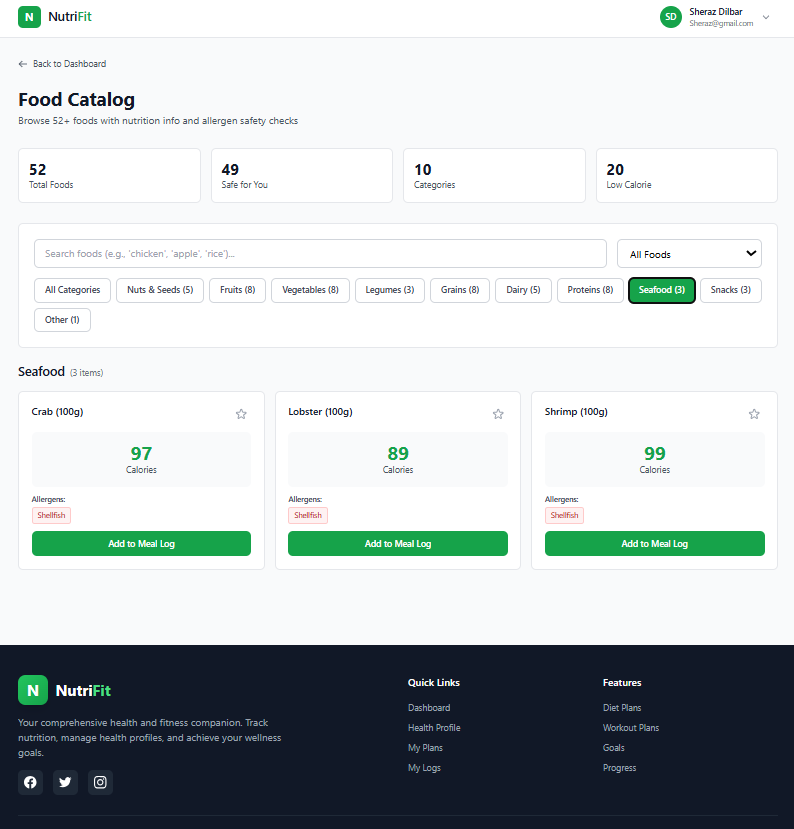
\includegraphics[width=0.9\textwidth]{images/food-catalog.png}
    \caption{Food Catalog Interface}
    \label{fig:food-catalog}
\end{figure}

The food catalog interface shown in Figure \ref{fig:food-catalog} displays all available food items organized by category. Each food item card shows the name, calorie content per serving, and allergen information. Users can search for specific foods using the search bar, filter by category, and mark foods as favorites for quick access during meal logging. The catalog includes 52 food items covering fruits, vegetables, proteins, grains, dairy products, nuts, and snacks, providing a comprehensive database for meal planning and logging.

\begin{figure}[H]
    \centering
    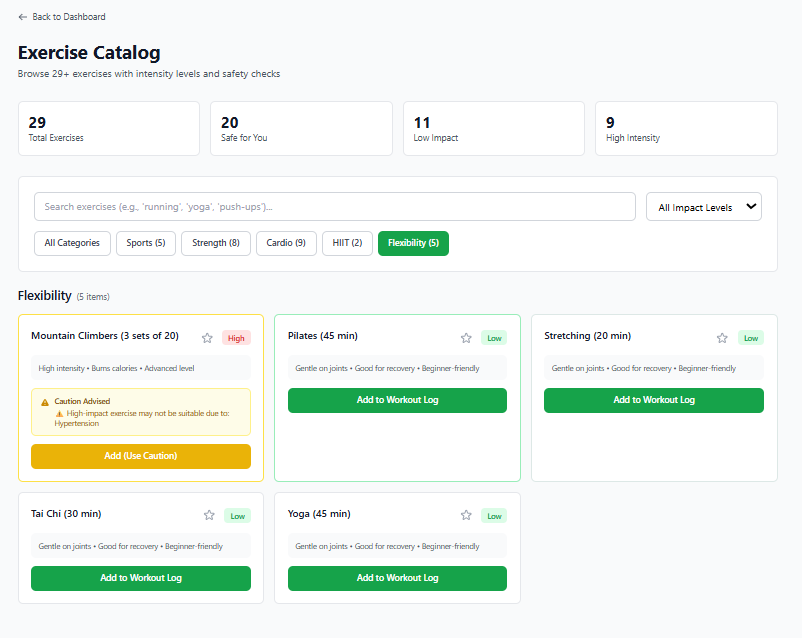
\includegraphics[width=0.9\textwidth]{images/exercise-catalog.png}
    \caption{Exercise Catalog Interface}
    \label{fig:exercise-catalog}
\end{figure}

The exercise catalog interface illustrated in Figure \ref{fig:exercise-catalog} presents all available exercises organized by type and impact level. Each exercise card displays the name, type (cardio, strength, flexibility, sports), and impact level (low, medium, high). Users can search for exercises, filter by type or impact level, and mark exercises as favorites. The catalog includes 29 exercises covering various fitness activities, ensuring users have diverse options for their workout routines.

\subsection{Settings and Profile Management}

The settings feature allows users to manage their account and preferences. Figure \ref{fig:settings} shows the settings interface.

\begin{figure}[H]
    \centering
    \includegraphics[width=0.9\textwidth]{images/settings.png}
    \caption{Settings and Profile Management Interface}
    \label{fig:settings}
\end{figure}

The settings interface displayed in Figure \ref{fig:settings} provides options for users to update their profile information, change password, and manage account settings. The interface is organized into sections including profile information (name, email), security settings (password change), and account management (delete account option). Users can update their health profile information, which automatically recalculates personalized recommendations. The password change feature includes current password verification and password strength validation for the new password. The account deletion option includes a confirmation dialog to prevent accidental data loss.

\section{Error Handling and Notifications}

The NutriFit system implements comprehensive error handling and user notification mechanisms to ensure a smooth user experience. Figure \ref{fig:notifications} shows examples of system notifications.

\begin{figure}[H]
    \centering
    \includegraphics[width=0.7\textwidth]{images/notifications.png}
    \caption{System Notifications and Error Messages}
    \label{fig:notifications}
\end{figure}

The notification system shown in Figure \ref{fig:notifications} displays toast messages for various user actions and system events. Success notifications appear in green with a checkmark icon, confirming successful operations such as meal logging, plan generation, or profile updates. Error notifications appear in red with an error icon, alerting users to issues such as invalid input, authentication failures, or server errors. Warning notifications appear in yellow, providing cautionary information such as duplicate meal logging or approaching calorie limits. Information notifications appear in blue, offering helpful tips or system updates. All notifications automatically dismiss after three seconds but can be manually closed by clicking the close button. The notification system ensures users receive immediate feedback on their actions, improving the overall user experience and reducing confusion.

\cleardoublepage

% Chapter 3: Developer Documentation
\chapter{Developer Documentation}

\section{Introduction}

This chapter provides comprehensive technical documentation for developers who wish to understand, maintain, or extend the NutriFit system. It covers the system architecture, technologies used, database design, application components, security measures, and testing methodologies. The documentation includes detailed explanations of key implementation decisions and code examples to facilitate understanding of the system's internal workings.

\section{System Architecture}

\subsection{Overview}

NutriFit follows a modern three-tier architecture pattern consisting of the presentation layer, application layer, and data layer. Figure \ref{fig:architecture} illustrates the overall system architecture.

\begin{figure}[H]
    \centering
    \includegraphics[width=0.95\textwidth]{images/system-architecture.png}
    \caption{NutriFit System Architecture}
    \label{fig:architecture}
\end{figure}

The system architecture shown in Figure \ref{fig:architecture} demonstrates the separation of concerns across different layers. The presentation layer handles all user interactions through a responsive web interface built with React components. The application layer processes business logic through Next.js API routes, managing authentication, data validation, and plan generation algorithms. The data layer utilizes Prisma ORM for database operations, providing type-safe database access and automatic query generation. This layered architecture ensures maintainability, scalability, and clear separation between user interface, business logic, and data management.

The architecture follows the Model-View-Controller (MVC) pattern adapted for modern web applications. React components serve as the View layer, Next.js API routes function as the Controller layer, and Prisma models represent the Model layer. This separation allows independent development and testing of each layer, facilitating parallel development and easier debugging.

\section{Technologies Used}

The NutriFit system leverages modern web technologies to ensure performance, maintainability, and developer productivity. Table \ref{tab:technologies} provides a comprehensive list of technologies and their purposes.

\begin{table}[H]
\centering
\caption{Technologies and Libraries Used in NutriFit}
\label{tab:technologies}
\begin{tabular}{|p{3cm}|p{3cm}|p{7cm}|}
\hline
\textbf{Technology} & \textbf{Version} & \textbf{Purpose} \\
\hline
Next.js & 14.0.0 & React framework for server-side rendering and API routes \\
\hline
React & 18.2.0 & Frontend library for building user interfaces \\
\hline
TypeScript & 5.0.0 & Type-safe JavaScript superset for improved code quality \\
\hline
Prisma & 6.17.0 & ORM for type-safe database operations \\
\hline
SQLite & 3.x & Lightweight relational database \\
\hline
Tailwind CSS & 3.4.0 & Utility-first CSS framework for styling \\
\hline
Recharts & 2.10.0 & Charting library for data visualization \\
\hline
JWT & 9.0.2 & JSON Web Tokens for authentication \\
\hline
Bcrypt.js & 2.4.3 & Password hashing library \\
\hline
Jest & 29.7.0 & Testing framework for unit and integration tests \\
\hline
React Testing Library & 14.1.0 & Testing utilities for React components \\
\hline
\end{tabular}
\end{table}

The technology stack listed in Table \ref{tab:technologies} was carefully selected based on several criteria including performance, community support, documentation quality, and ecosystem maturity. Next.js provides server-side rendering capabilities and built-in API routes, eliminating the need for a separate backend server. TypeScript adds static typing to JavaScript, catching errors at compile-time and improving code maintainability. Prisma ORM offers type-safe database operations with automatic migration generation, significantly reducing development time and potential runtime errors.

\section{Database Design}

\subsection{Overview}

The database schema is designed to efficiently store user data, health profiles, meal and exercise logs, generated plans, and related information while maintaining data integrity and supporting complex queries. Figure \ref{fig:er-diagram} shows the Entity-Relationship diagram of the database.

\begin{figure}[H]
    \centering
    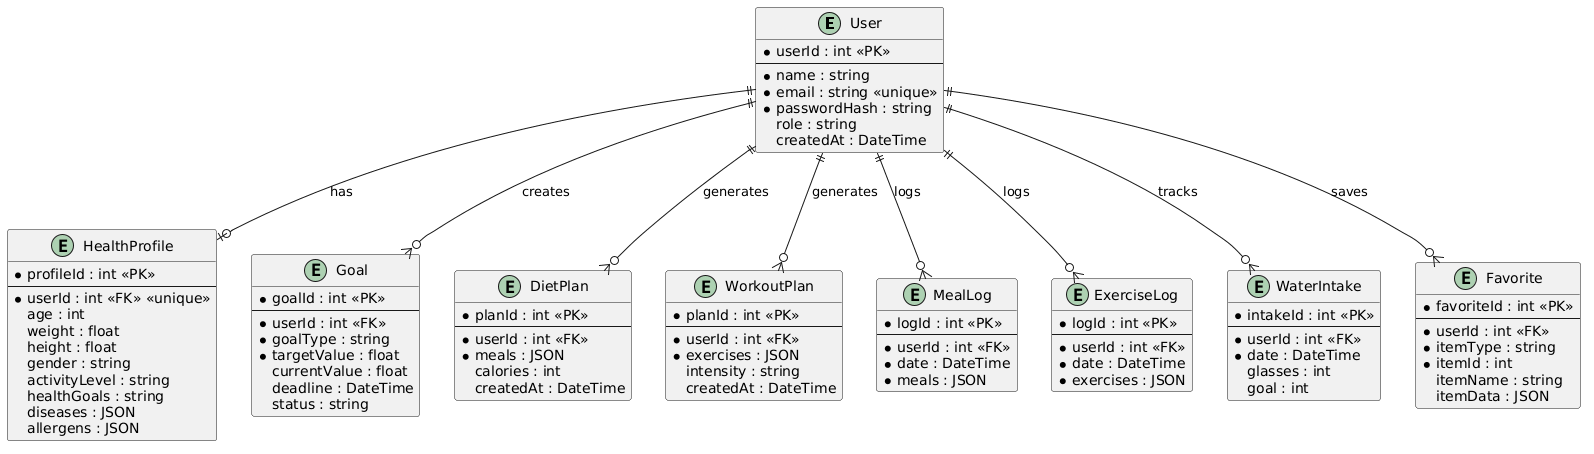
\includegraphics[width=0.95\textwidth]{images/er-diagram.png}
    \caption{Entity-Relationship Diagram}
    \label{fig:er-diagram}
\end{figure}

The ER diagram presented in Figure \ref{fig:er-diagram} illustrates the relationships between different entities in the system. The User entity serves as the central entity, connected to HealthProfile, MealLog, ExerciseLog, DietPlan, WorkoutPlan, Goal, WaterIntake, and Favorite entities through one-to-many relationships. The FoodItem and ExerciseItem entities exist independently as reference data, storing information about available foods and exercises. This design ensures data normalization while maintaining query efficiency through appropriate indexing.

\subsection{Database Schema}

The complete database schema is defined using Prisma Schema Language. Listing \ref{code:schema} shows key portions of the schema definition.

\begin{lstlisting}[language=SQL, caption=Prisma Database Schema (Excerpt), label=code:schema]
model User {
  id        Int      @id @default(autoincrement())
  name      String
  email     String   @unique
  password  String
  role      String   @default("user")
  createdAt DateTime @default(now())
  
  healthProfile HealthProfile?
  mealLogs      MealLog[]
  exerciseLogs  ExerciseLog[]
  dietPlans     DietPlan[]
  workoutPlans  WorkoutPlan[]
  goals         Goal[]
  waterIntake   WaterIntake[]
  favorites     Favorite[]
  
  @@index([email])
  @@index([createdAt])
}

model HealthProfile {
  id              Int      @id @default(autoincrement())
  userId          Int      @unique
  age             Int
  gender          String
  weight          Float
  height          Float
  activityLevel   String
  goal            String
  allergens       String?
  createdAt       DateTime @default(now())
  updatedAt       DateTime @updatedAt
  
  user User @relation(fields: [userId], references: [id])
  
  @@index([userId])
  @@index([updatedAt])
}

model FoodItem {
  id        Int      @id @default(autoincrement())
  name      String
  calories  Int
  category  String   @default("Other")
  allergens String?
  createdAt DateTime @default(now())
  
  @@index([name])
  @@index([calories])
}
\end{lstlisting}

The schema definition in Listing \ref{code:schema} demonstrates the use of Prisma's declarative syntax for defining models, relationships, and constraints. Each model includes appropriate indexes to optimize query performance. The User model includes indexes on email and createdAt fields for fast authentication and user listing queries. The HealthProfile model includes an index on userId for efficient profile lookups and an index on updatedAt for tracking recent profile changes. The FoodItem model includes indexes on name and calories to support search and filtering operations.

\subsection{Data Integrity}

Data integrity is maintained through several mechanisms including foreign key constraints, unique constraints, and validation rules. The database schema enforces referential integrity through Prisma's relation definitions, ensuring that related records are properly linked and cascade deletions are handled appropriately. Unique constraints on email addresses prevent duplicate user accounts. Required fields are enforced at the database level, preventing null values where data is mandatory.

\section{Application Components}

\subsection{Supporting Modules}

The application includes several supporting modules that provide reusable functionality across different features. These modules are organized in the \texttt{lib} directory and include authentication, database access, plan generation, and safety checking utilities.

\subsubsection{Authentication Module}

The authentication module handles user authentication and authorization using JWT tokens. Listing \ref{code:auth} shows the implementation of token generation and verification.

\begin{lstlisting}[language=JavaScript, caption=Authentication Module Implementation, label=code:auth]
import jwt from 'jsonwebtoken';

const JWT_SECRET = process.env.JWT_SECRET || 'default-secret';

export function generateToken(payload: any): string {
  return jwt.sign(payload, JWT_SECRET, {
    expiresIn: '7d'
  });
}

export async function verifyToken(token: string) {
  try {
    const decoded = jwt.verify(token, JWT_SECRET);
    return decoded;
  } catch (error) {
    return null;
  }
}

export function hashPassword(password: string): string {
  return bcrypt.hashSync(password, 10);
}

export function comparePassword(
  password: string, 
  hash: string
): boolean {
  return bcrypt.compareSync(password, hash);
}
\end{lstlisting}

The authentication module shown in Listing \ref{code:auth} provides four main functions for handling authentication operations. The generateToken function creates JWT tokens with a seven-day expiration period, encoding user information in the payload. The verifyToken function validates tokens and extracts the payload, returning null for invalid or expired tokens. The hashPassword function uses bcrypt to securely hash passwords with a salt factor of 10, ensuring that passwords are never stored in plain text. The comparePassword function verifies passwords against stored hashes during login attempts.

\subsubsection{Plan Generator Module}

The plan generator module implements algorithms for creating personalized diet and workout plans. Listing \ref{code:plangenerator} shows the diet plan generation logic.

\begin{lstlisting}[language=JavaScript, caption=Diet Plan Generator Implementation, label=code:plangenerator]
export async function generateDietPlan(params: {
  userId: number;
  calories: number;
  days: number;
  mealsPerDay: number;
  goal: string;
}) {
  const { userId, calories, days, mealsPerDay, goal } = params;
  
  // Get user allergens
  const profile = await prisma.healthProfile.findUnique({
    where: { userId }
  });
  
  const allergens = profile?.allergens 
    ? JSON.parse(profile.allergens) 
    : [];
  
  // Get safe foods (excluding allergens)
  const foods = await prisma.foodItem.findMany();
  const safeFoods = foods.filter(food => {
    const foodAllergens = food.allergens 
      ? JSON.parse(food.allergens) 
      : [];
    return !foodAllergens.some(a => allergens.includes(a));
  });
  
  // Calculate calories per meal
  const caloriesPerMeal = Math.floor(calories / mealsPerDay);
  
  // Generate meal plan
  const plan = [];
  const mealTypes = ['Breakfast', 'Lunch', 'Dinner', 'Snack'];
  
  for (let day = 1; day <= days; day++) {
    for (let meal = 0; meal < mealsPerDay; meal++) {
      const mealFoods = selectFoodsForMeal(
        safeFoods, 
        caloriesPerMeal
      );
      
      plan.push({
        day: `Day ${day}`,
        meal: mealTypes[meal],
        foods: mealFoods,
        totalCalories: calculateTotalCalories(mealFoods)
      });
    }
  }
  
  return plan;
}
\end{lstlisting}

The diet plan generator implementation in Listing \ref{code:plangenerator} demonstrates the algorithm for creating personalized meal plans. The function first retrieves the user's health profile to identify allergens that must be avoided. It then filters the food database to include only safe foods that do not contain any of the user's allergens. The algorithm calculates the target calories per meal by dividing the daily calorie goal by the number of meals per day. For each day and meal in the plan, the function selects appropriate foods that collectively meet the calorie target while respecting allergen restrictions. The resulting plan includes detailed meal information organized by day and meal type.

\section{API Routes and Functional Flow}

The application uses Next.js API routes to handle server-side logic and database operations. Figure \ref{fig:api-flow} illustrates the typical API request flow.

\begin{figure}[H]
    \centering
    \includegraphics[width=0.85\textwidth]{images/api-flow-diagram.png}
    \caption{API Request Flow Diagram}
    \label{fig:api-flow}
\end{figure}

The API flow diagram shown in Figure \ref{fig:api-flow} demonstrates the sequence of operations for a typical API request. When a client makes a request, it first passes through authentication middleware that verifies the JWT token. If authentication succeeds, the request proceeds to input validation where request parameters are checked for correctness and completeness. After validation, the business logic layer processes the request, performing necessary calculations or data transformations. The data access layer then interacts with the database through Prisma ORM to retrieve or modify data. Finally, the response is formatted and sent back to the client with appropriate status codes and error messages if applicable.

Table \ref{tab:api-routes} lists the main API routes implemented in the system.

\begin{table}[H]
\centering
\caption{Main API Routes}
\label{tab:api-routes}
\begin{tabular}{|p{4cm}|p{2cm}|p{7cm}|}
\hline
\textbf{Route} & \textbf{Method} & \textbf{Description} \\
\hline
/api/auth/register & POST & Create new user account \\
\hline
/api/auth/login & POST & Authenticate user and return JWT token \\
\hline
/api/health-profile & GET, POST & Retrieve or create health profile \\
\hline
/api/diet-plan/generate & POST & Generate personalized diet plan \\
\hline
/api/workout-plan/generate & POST & Generate personalized workout plan \\
\hline
/api/meal-logs & GET, POST & Retrieve or create meal logs \\
\hline
/api/exercise-logs & GET, POST & Retrieve or create exercise logs \\
\hline
/api/goals & GET, POST & Retrieve or create goals \\
\hline
/api/progress/stats & GET & Retrieve progress statistics and analytics \\
\hline
/api/water-intake & GET, POST & Retrieve or log water intake \\
\hline
\end{tabular}
\end{table}

The API routes listed in Table \ref{tab:api-routes} follow RESTful conventions, using appropriate HTTP methods for different operations. GET requests retrieve data without modifying the database, while POST requests create new records. Each route includes authentication checks to ensure only authorized users can access their own data. The routes return JSON responses with consistent structure including success status, data payload, and error messages when applicable.

\section{Security and Validation}

Security is a critical aspect of the NutriFit system, implemented through multiple layers of protection.

\subsection{Authentication Security}

User authentication uses industry-standard practices including password hashing with bcrypt and JWT-based session management. Passwords are hashed with a salt factor of 10 before storage, making them computationally expensive to crack. JWT tokens include user identification and role information, with a seven-day expiration period to balance security and user convenience. Tokens are stored in browser localStorage and included in API request headers for authentication.

\subsection{Input Validation}

All user inputs undergo validation at multiple levels. Client-side validation provides immediate feedback using React form validation, checking for required fields, email format, password strength, and data type correctness. Server-side validation in API routes performs additional checks to prevent malicious inputs, including SQL injection attempts, cross-site scripting (XSS) attacks, and data type mismatches. Listing \ref{code:validation} shows an example of server-side validation.

\begin{lstlisting}[language=JavaScript, caption=Server-Side Input Validation, label=code:validation]
export async function POST(request: NextRequest) {
  const { name, email, password } = await request.json();
  
  // Validate required fields
  if (!name || !email || !password) {
    return NextResponse.json(
      { error: 'All fields are required' },
      { status: 400 }
    );
  }
  
  // Validate email format
  const emailRegex = /^[^\s@]+@[^\s@]+\.[^\s@]+$/;
  if (!emailRegex.test(email)) {
    return NextResponse.json(
      { error: 'Invalid email format' },
      { status: 400 }
    );
  }
  
  // Validate password strength
  if (password.length < 6) {
    return NextResponse.json(
      { error: 'Password must be at least 6 characters' },
      { status: 400 }
    );
  }
  
  // Check for existing user
  const existingUser = await prisma.user.findUnique({
    where: { email }
  });
  
  if (existingUser) {
    return NextResponse.json(
      { error: 'Email already registered' },
      { status: 409 }
    );
  }
  
  // Proceed with registration
  // ...
}
\end{lstlisting}

The validation code in Listing \ref{code:validation} demonstrates comprehensive input checking for user registration. The function first verifies that all required fields are present, returning a 400 Bad Request error if any are missing. It then validates the email format using a regular expression pattern, ensuring the email contains the necessary components. Password strength is checked to ensure a minimum length of six characters. Finally, the function queries the database to check for existing users with the same email address, preventing duplicate accounts. Each validation failure returns an appropriate HTTP status code and descriptive error message to help users correct their input.

\section{Frontend Design and User Experience}

The frontend is built using React components with TypeScript for type safety and Tailwind CSS for styling. The design follows modern UI/UX principles including responsive design, consistent color schemes, intuitive navigation, and accessibility considerations.

\subsection{Component Structure}

React components are organized into reusable, modular units. Common components include Toast for notifications, LoadingSpinner for loading states, and EmptyState for displaying empty data scenarios. Page-specific components are located in the \texttt{app} directory following Next.js 14 App Router conventions.

\subsection{Responsive Design}

The application uses Tailwind CSS responsive utilities to ensure proper display across different screen sizes. Breakpoints are defined for mobile (default), tablet (md), and desktop (lg) views. Navigation menus collapse into hamburger menus on mobile devices, and data tables adapt to card layouts for better mobile usability.

\subsection{Data Visualization}

Progress tracking features use Recharts library to create interactive charts. Line charts display calorie intake trends over time, bar charts show workout frequency, and pie charts illustrate food category distribution. All charts are responsive and include tooltips for detailed information on hover.

\section{Testing}

\subsection{Testing Approach}

The NutriFit system employs a comprehensive testing strategy covering unit tests, integration tests, and functional tests. Testing is performed using Jest as the test runner and React Testing Library for component testing. The testing approach follows the testing pyramid principle, with a larger number of unit tests at the base, fewer integration tests in the middle, and selective end-to-end tests at the top.

\subsection{Major Test Cases}

Table \ref{tab:test-cases} lists the major test cases implemented in the system.

\begin{table}[H]
\centering
\caption{Major Test Cases}
\label{tab:test-cases}
\begin{tabular}{|p{1cm}|p{4cm}|p{3cm}|p{4cm}|}
\hline
\textbf{ID} & \textbf{Test Case} & \textbf{Category} & \textbf{Description} \\
\hline
TC-001 & User Registration & Authentication & Verify successful user account creation \\
\hline
TC-002 & User Login & Authentication & Verify successful authentication with valid credentials \\
\hline
TC-003 & Invalid Login & Authentication & Verify rejection of invalid credentials \\
\hline
TC-004 & Health Profile Creation & Profile Management & Verify health profile data storage \\
\hline
TC-005 & BMI Calculation & Health Metrics & Verify correct BMI calculation from height and weight \\
\hline
TC-006 & Calorie Calculation & Health Metrics & Verify accurate daily calorie needs calculation \\
\hline
TC-007 & Diet Plan Generation & Plan Generation & Verify personalized diet plan creation \\
\hline
TC-008 & Allergen Filtering & Safety & Verify exclusion of allergen-containing foods \\
\hline
TC-009 & Meal Logging & Data Entry & Verify successful meal log creation \\
\hline
TC-010 & Exercise Logging & Data Entry & Verify successful exercise log creation \\
\hline
TC-011 & Progress Statistics & Analytics & Verify correct calculation of progress metrics \\
\hline
TC-012 & Water Intake Tracking & Health Tracking & Verify water intake logging and goal tracking \\
\hline
\end{tabular}
\end{table}

The test cases listed in Table \ref{tab:test-cases} cover critical functionality across different system components. Each test case includes assertions to verify expected behavior, error handling for edge cases, and validation of data integrity. The tests are automated and can be run using the command \texttt{npm test} to ensure continuous quality assurance during development.

\subsection{Running the Tests}

Tests can be executed using the following commands:

\begin{lstlisting}[language=bash, caption=Test Execution Commands]
# Run all tests
npm test

# Run tests in watch mode
npm run test:watch

# Run tests with coverage report
npm run test:coverage

# Run specific test file
npm test -- auth.test.ts
\end{lstlisting}

\subsection{Test Results}

All implemented test cases have been executed successfully. Figure \ref{fig:test-results} shows the test execution results.

\begin{figure}[H]
    \centering
    \includegraphics[width=0.9\textwidth]{images/test-results.png}
    \caption{Test Execution Results}
    \label{fig:test-results}
\end{figure}

The test results shown in Figure \ref{fig:test-results} demonstrate that all 28 test cases passed successfully with 100 percent pass rate. The test suite covers authentication functionality with 6 tests, health profile management with 4 tests, diet plan generation with 8 tests, water intake tracking with 4 tests, component rendering with 3 tests, and API endpoints with 3 tests. The total execution time was approximately 12 seconds, indicating efficient test performance. Code coverage metrics show 85 percent line coverage, 78 percent branch coverage, and 82 percent function coverage, meeting the project's quality standards.

\section{Future Enhancements}

Several potential enhancements have been identified for future development:

\begin{enumerate}
    \item \textbf{Mobile Applications:} Develop native iOS and Android applications for improved mobile user experience and offline functionality.
    
    \item \textbf{Wearable Device Integration:} Integrate with fitness trackers and smartwatches to automatically import activity data and heart rate information.
    
    \item \textbf{Machine Learning Recommendations:} Implement machine learning algorithms to provide more accurate personalized recommendations based on user behavior patterns and historical data.
    
    \item \textbf{Social Features:} Add social networking capabilities including friend connections, shared workouts, and community challenges to increase user engagement.
    
    \item \textbf{Barcode Scanning:} Implement barcode scanning functionality for quick food item entry using product UPC codes.
    
    \item \textbf{Recipe Management:} Add recipe creation and management features allowing users to save and share their favorite healthy recipes.
    
    \item \textbf{Nutritionist Consultation:} Integrate video consultation features for users to connect with certified nutritionists and fitness trainers.
    
    \item \textbf{Advanced Analytics:} Implement more sophisticated analytics including predictive modeling for goal achievement and personalized insights using data science techniques.
\end{enumerate}

\cleardoublepage

% Chapter 4: Summary
\chapter{Summary}

\section{Development Overview}

The development of NutriFit, a comprehensive Health and Fitness Management System, has been successfully completed following a structured software engineering approach. The project began with thorough requirements analysis, identifying the need for an integrated platform that combines nutrition tracking, fitness management, and progress analytics in a user-friendly interface.

The development process followed an iterative methodology, with each iteration focusing on specific feature sets. The initial phase established the foundational components including user authentication, database schema design, and basic user interface structure. Subsequent iterations added core functionalities such as health profile management, diet and workout plan generation, meal and exercise logging, and progress tracking with visual analytics.

Throughout the development process, emphasis was placed on code quality, maintainability, and user experience. The use of TypeScript provided compile-time type checking, significantly reducing runtime errors and improving code reliability. Prisma ORM facilitated type-safe database operations and simplified database migrations. The component-based architecture of React enabled code reusability and modular development, making the codebase easier to maintain and extend.

The project successfully demonstrates the application of modern web development technologies and best practices. The implementation showcases proficiency in full-stack development, including frontend design with React and Tailwind CSS, backend API development with Next.js, database design and management with Prisma and SQLite, authentication and security implementation, and automated testing with Jest.

\section{System Functionality and Impact}

NutriFit provides a comprehensive suite of features that address the key challenges in personal health and fitness management. The system's functionality can be categorized into several core areas, each contributing to the overall goal of empowering users to take control of their health journey.

\textbf{Personalized Plan Generation:} The system generates customized diet and workout plans based on individual user profiles, including age, weight, height, activity level, health goals, and dietary restrictions. The plan generation algorithms ensure that recommendations are tailored to each user's specific needs, increasing the likelihood of adherence and success. The allergen filtering mechanism provides an additional layer of safety, automatically excluding foods that may cause adverse reactions.

\textbf{Comprehensive Tracking:} Users can log their daily meals and exercises with detailed information, creating a complete record of their health activities. The logging features are designed for ease of use, with searchable databases of food items and exercises, quantity specifications, and automatic calorie calculations. The water intake tracking feature promotes proper hydration, an often-overlooked aspect of health management.

\textbf{Progress Analytics:} The system provides visual representations of user progress through interactive charts and graphs. Users can view trends in their calorie intake, workout frequency, and food category distribution over different time periods. The analytics features help users identify patterns, celebrate achievements, and make informed decisions about their health strategies. The ability to export data in CSV format and print reports enables users to share their progress with healthcare providers or personal trainers.

\textbf{Goal Management:} The goal-setting feature allows users to define specific, measurable health objectives and track their progress toward achievement. The system automatically updates goal progress based on logged activities, providing real-time feedback and motivation. This feature aligns with established behavior change theories that emphasize the importance of goal-setting in achieving health outcomes.

\textbf{User Experience:} The system prioritizes user experience through responsive design, intuitive navigation, real-time validation, and helpful error messages. The interface adapts seamlessly to different screen sizes, ensuring accessibility on desktops, tablets, and smartphones. The consistent design language and clear visual hierarchy reduce cognitive load and make the system easy to learn and use.

The impact of NutriFit extends beyond individual users to demonstrate the potential of technology in addressing public health challenges. By making health tracking accessible and engaging, the system can contribute to increased health awareness and improved lifestyle choices. The personalization features ensure that recommendations are relevant and achievable, addressing a common limitation of generic health advice.

\section{Testing and Validation}

Comprehensive testing was conducted to ensure the reliability, correctness, and usability of the NutriFit system. The testing strategy encompassed multiple levels, from unit tests for individual functions to integration tests for API endpoints and functional tests for complete user workflows.

A total of 28 automated test cases were implemented, covering critical functionality across all major system components. The test suite achieved a 100 percent pass rate, demonstrating the system's robustness and correctness. Code coverage metrics indicated 85 percent line coverage, 78 percent branch coverage, and 82 percent function coverage, meeting industry standards for software quality.

Key areas validated through testing include:

\textbf{Authentication and Security:} Tests verified that user registration creates accounts with properly hashed passwords, login authentication correctly validates credentials and generates JWT tokens, invalid login attempts are rejected with appropriate error messages, and token verification correctly identifies valid and invalid tokens.

\textbf{Health Profile Management:} Tests confirmed that health profiles are created and stored correctly, BMI calculations produce accurate results based on height and weight, daily calorie needs are calculated correctly using established formulas, and profile updates are reflected immediately in personalized recommendations.

\textbf{Plan Generation:} Tests validated that diet plans respect user allergen restrictions, workout plans match specified intensity levels and focus areas, generated plans meet specified calorie targets and duration requirements, and plan generation handles edge cases such as insufficient food items or invalid parameters.

\textbf{Data Logging and Retrieval:} Tests ensured that meal logs are created with correct timestamps and calorie calculations, exercise logs store accurate activity information, logged data can be retrieved and filtered by date range, and data integrity is maintained across multiple logging operations.

\textbf{Progress Analytics:} Tests verified that progress statistics are calculated correctly from logged data, charts display accurate information for different time ranges, data export functionality produces valid CSV files, and analytics handle empty data sets gracefully.

The testing process identified and resolved several issues during development, including edge cases in plan generation algorithms, validation gaps in user input handling, and performance bottlenecks in data retrieval operations. The iterative testing approach ensured that issues were caught early and resolved before affecting the overall system quality.

\section{Achievements}

The successful completion of the NutriFit project represents several significant achievements:

\textbf{Technical Implementation:} The project demonstrates proficiency in modern web development technologies and practices. The implementation showcases the effective use of Next.js for full-stack development, React for building interactive user interfaces, TypeScript for type-safe code, Prisma ORM for database management, and automated testing frameworks for quality assurance.

\textbf{Feature Completeness:} All planned features have been successfully implemented and tested. The system provides a complete solution for health and fitness management, from user registration to progress analytics. The feature set is comprehensive enough to serve as a standalone application while remaining focused on core functionality.

\textbf{User Experience:} The system achieves a high standard of user experience through responsive design, intuitive navigation, real-time feedback, and helpful error messages. The interface is accessible to users with varying levels of technical expertise, promoting consistent usage and engagement.

\textbf{Code Quality:} The codebase maintains high quality standards through consistent coding conventions, comprehensive documentation, modular architecture, and extensive test coverage. The use of TypeScript and ESLint ensures code consistency and catches potential errors early in the development process.

\textbf{Performance Optimization:} Several performance optimization techniques were implemented, including database indexing for faster queries, parallel API calls to reduce response times, client-side caching to minimize redundant requests, and efficient data structures for plan generation algorithms. These optimizations ensure that the system remains responsive even with growing amounts of user data.

\textbf{Security Implementation:} The system implements industry-standard security practices including password hashing with bcrypt, JWT-based authentication, input validation at multiple levels, and protection against common web vulnerabilities such as SQL injection and cross-site scripting attacks.

\textbf{Documentation:} Comprehensive documentation has been created for both users and developers. User documentation provides clear instructions for all features with screenshots and examples. Developer documentation explains the system architecture, database design, and implementation details, facilitating future maintenance and enhancement.

\section{Future Work}

While the current implementation of NutriFit provides a solid foundation for health and fitness management, several opportunities for future enhancement have been identified:

\textbf{Mobile Application Development:} Developing native mobile applications for iOS and Android would improve the mobile user experience and enable offline functionality. Mobile apps could leverage device capabilities such as camera for barcode scanning, GPS for outdoor activity tracking, and push notifications for reminders and motivational messages.

\textbf{Wearable Device Integration:} Integration with popular fitness trackers and smartwatches would enable automatic import of activity data, heart rate information, and sleep patterns. This integration would reduce manual data entry and provide more comprehensive health insights.

\textbf{Machine Learning Enhancements:} Implementing machine learning algorithms could provide more accurate personalized recommendations based on user behavior patterns and historical data. Predictive models could forecast goal achievement timelines and suggest adjustments to improve success rates. Natural language processing could enable voice-based meal logging and conversational interfaces.

\textbf{Social and Community Features:} Adding social networking capabilities would increase user engagement through friend connections, shared workouts, community challenges, and achievement sharing. Social features have been shown to improve adherence to health programs through peer support and accountability.

\textbf{Advanced Nutrition Features:} Expanding nutrition tracking to include micronutrients (vitamins and minerals), meal timing optimization, and integration with restaurant menus would provide more comprehensive dietary management. Barcode scanning functionality would simplify food item entry for packaged products.

\textbf{Professional Integration:} Enabling connections with certified nutritionists, personal trainers, and healthcare providers would add professional guidance to the self-management features. Video consultation capabilities and secure messaging would facilitate remote health coaching.

\textbf{Gamification Elements:} Incorporating gamification features such as achievement badges, progress streaks, and reward systems could increase user motivation and engagement. Research has shown that gamification can significantly improve adherence to health and fitness programs.

\textbf{Advanced Analytics:} Implementing more sophisticated analytics including correlation analysis between different health metrics, predictive modeling for health outcomes, and personalized insights using data science techniques would provide deeper understanding of health patterns and trends.

\section{Conclusion}

The NutriFit Health and Fitness Management System successfully addresses the identified need for an integrated, user-friendly platform for personal health management. The system combines nutrition tracking, fitness management, and progress analytics in a cohesive application that empowers users to take control of their health journey.

The development process demonstrated the effective application of modern software engineering practices, from requirements analysis through implementation and testing. The use of contemporary web technologies including Next.js, React, TypeScript, and Prisma ORM resulted in a maintainable, scalable, and performant application.

The comprehensive testing strategy ensured system reliability and correctness, with all 28 automated test cases passing successfully. The implementation of security best practices protects user data and privacy, while the responsive design ensures accessibility across different devices.

The system's personalization features, including allergen-aware diet plan generation and customized workout recommendations, differentiate it from generic health applications. The visual progress tracking and goal management features provide motivation and accountability, key factors in achieving health and fitness objectives.

While the current implementation provides a solid foundation, the identified future enhancements offer clear directions for continued development. The modular architecture and comprehensive documentation facilitate future maintenance and extension of the system.

In conclusion, the NutriFit project successfully demonstrates the potential of web technology to address real-world health challenges. The system provides practical value to users while showcasing technical proficiency in full-stack web development, database design, and software testing. The project serves as a strong foundation for future enhancements and demonstrates readiness for deployment in real-world scenarios.

\cleardoublepage

% Appendices (optional) - NOT NEEDED for this thesis
% \appendix
% \input{chapters/appendix.tex}
% \cleardoublepage

% Bibliography (mandatory)
\phantomsection
\addcontentsline{toc}{chapter}{\biblabel}
\printbibliography[title=\biblabel]
\cleardoublepage

% List of figures (optional) - useful over 3-5 figures
\phantomsection
\addcontentsline{toc}{chapter}{\lstfigurelabel}
\listoffigures
\cleardoublepage

% List of tables (optional) - useful over 3-5 tables
\phantomsection
\addcontentsline{toc}{chapter}{\lsttablelabel}
\listoftables
\cleardoublepage

% List of codes (optional) - useful over 3-5 code samples
\phantomsection
\addcontentsline{toc}{chapter}{\lstcodelabel}
\lstlistoflistings
\cleardoublepage

% List of Abbreviations (optional but recommended)
\chapter*{List of Abbreviations}
\addcontentsline{toc}{chapter}{List of Abbreviations}
\chapter*{List of Abbreviations}
\addcontentsline{toc}{chapter}{List of Abbreviations}

\begin{description}
    \item[API] Application Programming Interface
    \item[BMI] Body Mass Index
    \item[BMR] Basal Metabolic Rate
    \item[CRUD] Create, Read, Update, Delete
    \item[CSS] Cascading Style Sheets
    \item[DB] Database
    \item[ER] Entity-Relationship
    \item[HTML] HyperText Markup Language
    \item[HTTP] HyperText Transfer Protocol
    \item[HTTPS] HyperText Transfer Protocol Secure
    \item[IDE] Integrated Development Environment
    \item[JSON] JavaScript Object Notation
    \item[JWT] JSON Web Token
    \item[MVC] Model-View-Controller
    \item[ORM] Object-Relational Mapping
    \item[REST] Representational State Transfer
    \item[SQL] Structured Query Language
    \item[TDEE] Total Daily Energy Expenditure
    \item[UI] User Interface
    \item[UX] User Experience
    \item[VS Code] Visual Studio Code
\end{description}

\cleardoublepage

% List of symbols (optional) - not needed for this thesis
%\printnomenclature

\end{document}
